\documentclass[11pt,a4paper]{article}
%\usepackage[utf8]{inputenc}
%\usepackage[ascii]{inputenc}
\usepackage{geometry}
\usepackage[dvipsnames]{xcolor}
\usepackage{textcomp}
\usepackage{graphicx}
\usepackage{caption}
\usepackage{subcaption}
\usepackage{amsmath}
\usepackage{tikz}

\begin{document}

\tableofcontents

\section*{Introduction}
Objectif du cours : 
\begin{itemize}
\item Rappel des notions de bases de traitement du signal 
\item Design et synthèse de filtre 
\item Applications sous MATLAB/GNU Octave
\end{itemize}

Ce cours sera principalement formulé sous forme de réponse à des questions précises généralement couplées à des questions techniques sur le sujet.

\section{Fondamentaux}
\subsection{Traitement du signal}
Le traitement du signal est le champ de l'ingénierie qui concerne les outils physiques et mathématiques mis en œuvre pour la transmission de l'information suivant des contraintes précises.\\

On peut définir le signal de la façon suivante: "Le signal est le support de l’information émise par une source et destinée à un récepteur." (M. Bellanger, \textit{Traitement numérique du signal, 2012}). La problématique de base étant que, bien souvent, l'information peut voir son contenu dégradé par divers mécanismes entre la source et le récepteur. Le traitement du signal, qu'il soit analogique ou numérique, va alors souvent consister à extraire ou conserver l'information entre ces deux points d'intérêt.\\

L'information peut ici prendre plusieurs formes physiques différentes. Il peut s'agir d'une onde électromagnétique se propageant dans le vide, l'air ou encore un cable. Il peut également s'agir d'un champ de pression ou de déformation. L'information peut également être "codée" comme c'est le cas des signaux numériques par opposition aux signaux analogiques.\\

\textbf{Question: Exemple de traitement du signal analogique et numérique dans la vide quotidienne ?}\\

Le traitement du signal est basé sur la connaissance des mécanismes physiques à l’œuvre dans la propagation du signal (acoustique, électromagnétisme, etc...) et sur des outils mathématiques (statistiques, analyse de fonctions) permettant à la fois d'extraire des caractéristiques du signal ou de les modifier de manière contrôlée. Cette opération est souvent réalisée à l'aide de ce qu'on appelle des filtres. \\
 
\subsection{Qu'est ce qu'un filtre ?}
"En traitement du signal, un filtre est un dispositif ou un processus permettant de retirer des composantes ou des parties indésirables d'un signal." (/en.wikipedia.org/wiki/Filter (signal processing))\\

\vspace{0.5cm}

\begin{center}
	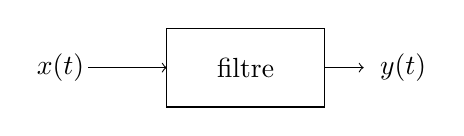
\begin{tikzpicture}
	%\draw (2.15,-1.5) node {Glc};
	%\draw[->] (2.15,-1)-- (2.15,-0.5);
	%\draw (1.25,-0.5) rectangle(3,0.5);
	\draw (2.15,0) node {$x(t)$};
	%\draw[->] (2.15,0.5)-- (2.15,1);
	%\draw (2.15,1.5) node {ATP};
	
	\draw[->] (2.5,0)-- (3.5,0);
	\draw (3.5,-0.5) rectangle(5.5,0.5) ;
	\draw (4.5,0) node {filtre};
	%\draw[->] (4.5,0.5) arc(90:60:0.5);
	%\draw[->] (4.5,-0.5) arc(-90:-120:0.5);
	%\draw[->] (4.5,-1)-- (4.5,-0.5);
	%\draw (4.5,-1.5) node {Glt};
	%\draw[->] (4.5,0.5)-- (4.5,1);
	%\draw (4.5,1.5) node {ATP};
	
	\draw[->] (5.5,0)-- (6,0);
	%\draw[->] (6,-0.5) rectangle(7,0.5); 
	\draw (6.5,0) node {$y(t)$};
	%\draw[->] (6.5,-1)-- (6.5,-0.5);
	%\draw (6.5,-1.5) node {O$_2$};
	%\draw[->] (6.5,0.5)-- (6.5,1);
	%\draw (6.5,1.5) node {ATP};
	\end{tikzpicture}
\end{center}

\vspace{0.5cm}

On note que, dans le cadre plus large de l'ingénierie des systèmes, ce formalisme entrée-sortie est régulièrement employé comme par exemple en automatique, où le but est cette fois d'arriver à obtenir une variable de sortie précise en agissant sur la variable d'entrée. D'ailleurs, les éléments de bases du formalisme mathématique sont les mêmes. Qu'il s'agisse d'un "filtre" ou d'un "système" la base théorique a pour objectif de prédire la réponse du système. Cette notion de prédiction/traitement/commande amène naturellement à la grande question suivante.

\subsection{Comment caractériser un filtre ou un système ?}  
\textbf{Question: Quelles notions/mots clés sont associées pour vous à la caractérisation d'un filtre ou d'un système ?}\\

De nombreuses notions plus ou moins intuitives peuvent être employées pour décrire l'action, souhaitée ou effective, d'un filtre/système, et ces dernières sont souvent au cœur de la conception du filtre/système en question.\\

La notion la plus évidente, déjà abordée par le passé, est la question analogique/numérique. Et cette première subdivision en conditionne d'autres. Dans le cas des signaux analogiques, on distingue régulièrement les filtres "actifs" des filtres "passifs". Un filtre actif est un filtre qui utilise une source d'énergie externe pour amplifier tout ou partie du signal. L'objectif est souvent d'obtenir un meilleur rapport signal-sur-bruit. Dans le cas des filtres numériques, on peut prendre comme premier exemple la notion de causalité. Un filtre numérique non-causal est un filtre qui va utiliser des échantillons du "futur" dans son algorithme de traitement. Un tel filtre ne peut évidemment effectuer un traitement en temps réel et n'est réalisable qu'à l'aide d'une mémoire embarquée associée.\\

Mais avant ces deux notions plutôt intuitives, il y a deux caractéristiques importantes des filtres qui sous-tendent une grande partie des outils mathématiques présentés dans ce cours. Au vu de leur importance globale et de leur aspect moins intuitif (car plus mathématique et calculatoire) on prendra le temps de présenter et de discuter en détail ces deux notions: la \textbf{linéarité} et l'\textbf{invariance dans le temps}.

\subsection{Notion de linéarité}
\textbf{Question: Que veut dire linéaire en ingénierie des systèmes/automatique/traitement du signal ?}\\

La notion de linéarité est un concept majeur en mathématiques et aussi en physique où l'outil mathématique est régulièrement utilisé. Elle peut s'écrire mathématiquement comme suit: soit $f$ une fonction 1D d'une variable réelle,  et soit $x_1$ et $x_2$ et $a$, trois nombres réels, alors:

\[f(a x_1 + x_2) = a f(x_1) + f(x_2)  \] 

\textbf{Linéarité : application}
\textbf{Soit $x$ une variable réelle, les fonctions suivantes sont-elles linéaires ?}:
\begin{itemize}
\item $f(x) = a x^2 + b x + c$ (avec $a$, $b$ et $c$ des constantes réelles positives) 
\item $f(x) = \sqrt{x^2}$
\item $f(x) = a$
\item $f(x) = \ln(x)$
\item $f(x) = \frac{1}{a x + b}$
\end{itemize}

Maintenant que le concept de linéarité a été introduit et/ou rappelé, on peut discuter de son importance en physique et ingénierie. Dans ces deux domaines on se place soit dans un cas linéaire, soit on traite l'objet d'étude de façon à rendre au moins partiellement applicable l'hypothèse de linéarité. En physique cela implique qu'on utilise régulièrement la notion de développement limité. L'un des usages des développement limités étant de remplacer une fonction non linéaire par une approximation linéaire de cette dernière afin de faciliter les calculs.\\

En résumé, si un système est linéaire, la décomposition de son signal de sortie comme somme d'entrée élémentaire est pertinente. Ce qui va s'avérer important plus tard notamment lorsque la théorie de Fourier entrera en jeu.

\subsection{Notion d'invariance dans le temps}
Afin de discuter la notion d'invariance dans le temps il est utile de rappeler la notion de retard ou décalage temporel d'une fonction sous sa forme mathématique.\\

\textbf{Question: Comment s'exprime la notion de retard en mathématiques ?}\\

Un exemple simple est de prendre la fonction exponentielle: exp$(x)$. On sait que exp$(0) = 1$ et exp$(1) = e$. Si on s'intéresse maintenant à la fonction exp$(x-\tau)$ et qu'on recherche les mêmes points particuliers, on retrouve la valeur 1 pour $x = \tau$ et la valeur $e$ pour $x= \tau + 1$. On se rend compte qu'en remplaçant exp$(x)$ par exp$(x-\tau)$, on décale la fonction de $\tau$ suivant les $x$ croissants.  

De façon plus générale, soit $f$ une fonction d'une variable réelle $x$. alors la fonction $g(x) = f(x-\tau)$ correspond à $f(x)$ avec un retard $\tau$. Cette définition correspond aux fonctions continues mais s'applique de façon analogue aux signaux discrets. L'équivalent discret d'une fonction est généralement appelé "suite". Soit $u(n)$, une suite pouvant représenter un signal, la suite $u(n-m)$, où $m$ est un entier, correspond à la suite $u(n)$ décalée de $m$ échantillons. \\

L'invariance dans le temps d'un filtre/système s'exprime alors de la façon suivante: Soit un filtre/système faisant correspondre une sortie $y(t)$ à une entrée $x(t)$. Soit $\tau$ un réel, le filtre/système est dit invariant dans le temps si quelque soit $\tau$, le système fait correspondre la sortie $y(t-\tau)$ à l'entrée $x(t-\tau)$.\\

On peut reformuler en disant que la réponse d'un filtre/système invariant dans le temps ne doit pas dépendre du moment où on l'utilise.\\

\subsection{Capteur linéaire et invariant dans le temps}
Un autre domaine très lié au traitement du signal et où la linéarité est importante est le domaine des \textbf{capteurs}. Un capteur peut être défini de la façon suivante: "Dispositif permettant de capter un phénomène physique et de le restituer sous forme de signal."(Dictonnaire "Le Robert") ou encore comme "Un capteur est un dispositif transformant l'état d'une grandeur physique observée en une grandeur utilisable, telle qu'une tension électrique, une hauteur de mercure, un courant électrique ou la déviation d'une aiguille."\\

\textbf{Question: Que vous évoque la notion de linéarité d'un capteur ?}\\

La linéarité d'un capteur est équivalente à celle présentée pour celle d'un filtre/système. Si on injecte la somme de deux signaux d'entrée $x_1(t)$ et $x_2(t)$, alors la sortie mesurée doit être la somme des sorties $y_1(t)$ et $y_2(t)$ qu'on mesurerait séparément. Dans les faits, un grand nombre de capteurs ne remplissent cette condition que sur une certaines plages de valeur d'entrée.\\

\textbf{Discussion: Plage de linéarité : exemple du ressort}

\subsection{Système linéaire et invariant dans le temps, et réponse impulsionnelle}
Pour démarrer cette partie, on doit définir la notion d'impulsion de Dirac noté $\delta(t)$. Cette dernière peut être vu que comme le cas limite mathématique d'une impulsion de largeur finie. Sur un plan purement mathématique la distribution de Dirac (et la notion de distribution en général) permet de définir la dérivée de fonction comme l'échelon de Heaviside.  De cette définition mathématique découle une possibilité très signifiante dans le cadre de l'ingénierie des systèmes. Elle permet, pour les systèmes linéaires  et invariants dans le temps, d'écrire la relation suivante:\\  
 
\[y(t) = \int^{\infty}_{-\infty} h(\tau) x(t-\tau) \; d\tau = h(t) \star x(t)\] \\

Où $y(t)$ est le signal de sortie, $x(t)$ celui d'entrée et $h(t)$ la réponse impulsionnelle du système. La réponse impulsionnelle du système est défini comme la sortie d'un système lorsque celui reçoit une impulsion de Dirac en entrée.

\begin{center}
	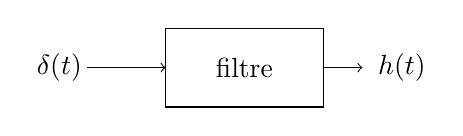
\begin{tikzpicture}

	\draw (2.15,0) node {$\delta(t)$};

	\draw[->] (2.5,0)-- (3.5,0);
	\draw (3.5,-0.5) rectangle(5.5,0.5) ;
	\draw (4.5,0) node {filtre};

	
	\draw[->] (5.5,0)-- (6,0);
	\draw (6.5,0) node {$h(t)$};

	\end{tikzpicture}
\end{center}

Cette équation est appelée \textbf{équation de convolution du filtre}, puisque, comme le montre le membre de droite de l'équation précédente, la sortie du filtre s'écrit comme le produit de convolution du signal d'entrée et de la \textbf{réponse impulsionnelle du filtre}. Les équations précédentes sont valables pour les fonctions continues. Un équivalent existe dans le domaine discret: \\

\[y(n) = \Sigma^{\infty}_{-\infty} h(m) x(n-m) = h(n) \star x(n)\]\\

Les fonctions d'entrée et de sortie et la réponse impulsionnelle, sont alors remplacées par des suites et l'intégrale, somme continue, est remplacée par une somme discrète. Un derniers point est la fonction de Dirac qui dans le domaine discret a pour équivalent \textbf{l'impulsion de Kronecker}\\ 

Les concepts mathématiques introduits dans les paragraphes précédents constituent la base sur laquelle reposent presque intégralement les notions qui vont être présentées dans les sections suivantes de ce cours.

\subsection{Transformée de Laplace} 

\textbf{Question: Que vous évoque la transformée de Laplace ? à quoi sert-elle ?}\\

La transformée de Laplace qui transforme une fonction (ici $f$) d'une \textbf{variable réelle} (ici $t$) en une fonction $L{f}$ d'une \textbf{variable complexe} (ici $p$) et définie par la relation mathématique suivante :

\[L{f}(p) = \int^{\infty}_{0} f(t) e^{-pt} \; dt\] 

Avant d'aller plus loin dans le développement mathématique de cette notion, on va d'abord évoquer son utilité. L'intérêt principal de la transformée de Laplace est de simplifier des opérations mathématiques. Elle permet notamment de remplacer une opération de \textbf{convolution} entre deux fonctions par une multiplication. Elle permet également de simplifier la résolution d'un grand nombre d'équations différentielles ordinaires. On peut être tenté de dire que le problème est simplement déplacé, puisqu'au lieu d'intégrer l'équation différentielle en elle-même on calcule une autre intégrale pour obtenir sa transformée. Cependant il faut comprendre que l'obtention de la transformée est souvent bien plus simple que le calcul direct, et ce car les transformées d'un grand nombre de fonctions sont connues.\\

Pour donner un peu de sens à tout cela, les transformées de Laplace de quelques fonctions usuelles vont être calculées. Ce calcul explicite a plus pour but de manipuler les concepts et les outils mathématiques. Par la suite les transformées seront dans un tableau qu'on pourra consulter quand elle ne seront pas directement calculées par  ordinateur.\\

\textbf{Exercice: Calculer les transformées de Laplace suivantes}\\

\begin{itemize}
\item $\delta (t)$ (impulsion de dirac) 
\item $u(t)$ (échelon de heaviside)
\item $r(t) = t$ (rampe)
\item $f(t) = e^{-at}$ (exponentielle décroissante)
\item $sin(\omega t)$
\end{itemize}

\paragraph{\textbf{1.} $\delta (t)$}
\[L{\delta}(p) = \int^{\infty}_{0} \delta(t) e^{-pt} \; dt = 1\] 
La démonstration de cette dernière est laissée de côté à cause des spécificités de la distribution de Dirac et de la nature de la transformée de Laplace. Ceci requiert donc beaucoup d'étape pour être rigoureux pour obtenir cela dit un résultat relativement facile à intuiter, si on sait que $\int^{\infty}_{-\infty}f(\tau)\delta(\tau) d\tau = f(0)$

\paragraph{\textbf{2.} $u (t)$}
On définit $u(t)$ comme la fonction nulle si $t < 0$ et égale à sinon:

\begin{center}
	\begin{tikzpicture}

	\draw[->] (0,0)-- (5,0);
	\draw (2.5,-0.25) node {0};
	\draw[->] (2.5,0)-- (2.5,3);
	\draw (5.5,0.25) node {$t$};
	\draw (2.5,3.5) node {$u(t)$};
	\draw (2.25,2) node {1};
	
	\draw[thick,blue] (0,0)-- (2.5,0);
	\draw[thick,blue] (2.5,0)-- (2.5,2);
	\draw[thick,blue] (2.5,2)-- (5,2);

	\end{tikzpicture}
\end{center}

Sa transformée de Laplace s'écrit donc comme suit :

\[L{u}(p) = \int^{\infty}_{0} u(t) e^{-pt} \; dt\] 

Suivant la définition de la fonction on peut alors écrire : 

\[L{u}(p) = \int^{\infty}_{0} e^{-pt} \; dt =  \Big[-\frac{e^{-pt}}{p}\Big]^{\infty}_{0} = \frac{-e^{-p \infty}}{p} + \frac{e^{-p 0}}{p} = \frac{1}{p}  \] 

On rappelle ici que $p$ est un nombre \textbf{complexe}.

\paragraph{\textbf{3.} $r(t)$}
La fonction r(t) est la fonction rampe définie comme une droite de pente 1 sur les réels positifs.

\begin{center}
	\begin{tikzpicture}

	\draw[->] (0,0)-- (5,0);
	\draw (2.5,-0.3) node {0};
	\draw[->] (2.5,0)-- (2.5,3);
	\draw (5.5,0.25) node {$t$};
	\draw (2.5,3.5) node {$r(t)$};
	\draw (2.25,2) node {1};
	\draw (4.5,-0.3) node {1};
	
	\draw[thick,blue] (0,0)-- (2.5,0);
	\draw[thick,blue] (2.5,0)-- (4.5,2);
	%\draw[thick,blue] (2.5,2)-- (5,2);

	\end{tikzpicture}
\end{center}


On suit les mêmes étapes que précédemment : 

\[L{u}(p) = \int^{\infty}_{0} t e^{-pt} \; dt\]

Le calcul de cette transformée est un peu plus complexe. Il fait appel au théorème de l'intégration par parties:

\[\int^{b}_{a} u(t) v'(t) \; dt =  u(b) v(b)-u(a) v(a) -\int^{b}_{a} u'(t) v(t) \; dt  \] 

De façon plus explicite, si on doit intégrer un produit de fonction, dont on connaît les dérivées et les primitives on peut décomposer l'intégrale du produit en deux parties plus simples à calculer. Donc ici :

\[L{r}(p) = \int^{\infty}_{0} t e^{-pt} \; dt =  \Big[-\frac{te^{-pt}}{p}\Big]^{\infty}_{0} + \int^{\infty}_{0} \frac{e^{-pt}}{p} \; dt\]

\[ \Big[-\frac{te^{-pt}}{p}\Big]^{\infty}_{0} = 0\]

\[ \int^{\infty}_{0} \frac{e^{-pt}}{p} \; dt = \Big[-\frac{te^{-pt}}{p^2}\Big]^{\infty}_{0} = \frac{1}{p^2}\]

\[ L{r}(p) = \int^{\infty}_{0} t e^{-pt} \; dt  = \frac{1}{p^2}\]

\paragraph{\textbf{4.} $f(t) = e^{-at}$}
Cette fonction est fréquemment rencontrée en ingénierie car elle constitue la réponse typique d'un système premier ordre, comme par exemple la décharge d'un condensateur dans un circuit RC simple.
\begin{center}
	\begin{tikzpicture}

	\draw[->] (0,0)-- (5,0);
	\draw (2.5,-0.3) node {0};
	\draw[->] (2.5,0)-- (2.5,3);
	\draw (5.5,0.25) node {$t$};
	\draw (2.5,3.5) node {$f(t)$};
	\draw (2.25,2) node {1};
	\draw (2.05,0.37*2) node {1/e};
	\draw[dashed] (2.5,0.37*2)-- (3.5,0.37*2);
	\draw (3.5,-0.3) node {1/a};
	\draw[dashed] (3.5,0.37*2)-- (3.5,0);
	%\draw (4.5,-0.3) node {1};
	
	%\draw[thick,blue] (0,0)-- (2.5,0);
	%\draw[thick,blue] (2.5,0)-- (4.5,2);
	%\draw[thick,blue] (2.5,2)-- (5,2);
	\draw[domain=2.5:5,color=blue] plot (\x,{2*exp(-\x+2.5)});

	\end{tikzpicture}
\end{center}


Cette transformée est plus simple à calculer car elle se base sur le calcul de la première.

\[L{f}(p) = \int^{\infty}_{0} e^{-at} e^{-pt} \; dt\]

Si on réécrit $e^{-at} e^{-pt}$ comme $e^{-(p+a)t}$, il vient directement que: 

\[L{f}(p) = \frac{1}{p+a}\]

Il est intéressant de noter que, si on multiplie une fonction par $f(t) = e^{-at}$, quelque soit, la fonction cela induit que $p$ va devenir $p+a$ dans la transformée de Laplace.

\paragraph{\textbf{5.} $f(t) = \sin(\omega_0 t)$}
Pour trouver cette transformer, on peut utiliser deux méthodes: L'intégration par parties ou bien une des formules d'Euler. Les formules d'Euler établissent le lien entre les exponentielles complexes et les fonctions trigonométriques sin et cos:  $\sin(\omega_0 t) = \frac{e^{j \omega_0 t} - e^{-j \omega_0 t}}{2j}$

\[L{f}(p) = \int^{\infty}_{0} \sin(\omega_0 t) e^{-pt} \; dt =  \int^{\infty}_{0} \frac{e^{j \omega_0 t} - e^{-j \omega_0 t}}{2j} e^{-pt} \; dt\]

On peut alors réécrire l'ensemble comme :

\[L{f}(p) =  \int^{\infty}_{0} \frac{e^{j \omega_0 t}e^{-pt}}{2j}  \; dt - \int^{\infty}_{0} \frac{e^{-j \omega_0 t}e^{-pt}}{2j}  \; dt = \frac{1}{2j}\Big[\frac{2j\omega_0}{p^2 + \omega_0^2}  \Big] = \frac{\omega_0}{p^2 + \omega_0^2} \]

\subsubsection{Propriétés de la transformée de Laplace}
Dans cette section, les propriétés utiles dans le transformée de Laplace vont être abordées.

\textbf{Exercices : } 

\[L{af+g}(p) = \int^{\infty}_{0}( a f(t) + g(t)) e^{-pt} \; dt = \; ?\]

Avec le résultat de ce calcul on observe la notion de linéarité.

\[L{f'}(p) = \int^{\infty}_{0}f'(t) e^{-pt} \; dt = \; ?\]

Ici en réutilisant l'intégration par partie on déduit une règle générale pour la transformée d'une dérivée.\\

Soit $F(t) = \int^{t}_{0} f(\tau)  \; d\tau$,

\[L{F}(p) = \int^{\infty}_{0}F(t) e^{-pt} \; dt = \; ?\]

Pour finir, un des intérêts principaux de ces transformées est sa relation avec la convolution.

soit deux fonctions $f(t)$ et $g(t)$ et $f \star g$ le produit de convolution de ces fonctions, alors on peut écrire :

\[L (f \star g) (p) =  \int^{\infty}_{0}(f \star g) e^{-pt} \; dt = L(f)L(g) (p)  \]

%Par application du théorème de Fubini, on peut écrire:

%\[L (f \star g) (p) =  \int^{\infty}_{0}(f \star g) e^{-pt} \; dt =  (\int^{\infty}_{0}(f) e^{-pt} \; dt ) (\int^{\infty}_{0}(g) e^{-pt} \; dt)  \]

\subsection{Série de Fourier, Transformée de Fourier et lien avec la transformée de Laplace}
L'objectif de cette-sous partie est de compléter un peu les concepts présentés précédemment sur la transformée de Laplace et d'illustrer la construction mathématique de la théorie de Fourier. On verra que comprendre celle-ci permet également de mieux saisir certains aspects du traitement du signal numérique.

\subsubsection{Séries de Fourier}
Les séries de Fourier sont un outil d'étude des fonctions périodiques. On peut les voir comme la mise en œuvre mathématique du principe suivant :\\

\textbf{Toute fonction périodique de période $T$, peut s'écrire comme une somme pondérée de fonctions sinusoïdales de période $T$}\\

Ce qui, pour une fonction $s(t)$ de période $T$, se traduit par la formule mathématique suivante: 

\[ s(t) = \overset{+\infty}{\underset{n = -\infty}{ \Sigma}} c_n(s)e^{i 2\pi \frac{n}{T}t}\]

où $n$ est un entier, où $c_n(s)$

\[ c_n(s) = \frac{1}{T} \int_{T} f(t)e^{i 2\pi \frac{n}{T}t} \; dt \]
% mettre cos et sin
Soit les quatres fonctions suivantes : 
\begin{enumerate}
\item $g_1(t) = \cos(2 t)$
\item $g_2(t) = 0.55 \cos(2 t) + 0.45 \cos(4 t)$
\item $g_3(t) = 0.6 \cos(2 t) + 0.3 \cos(4 t) + 0.1 \cos(6 t)$
\item $g_4(t) = 0.4 \cos(2 t) + 0.3 \cos(4 t) + 0.2 \cos(6 t) + 0.1 \cos(8 t) $
\end{enumerate}

\begin{center}
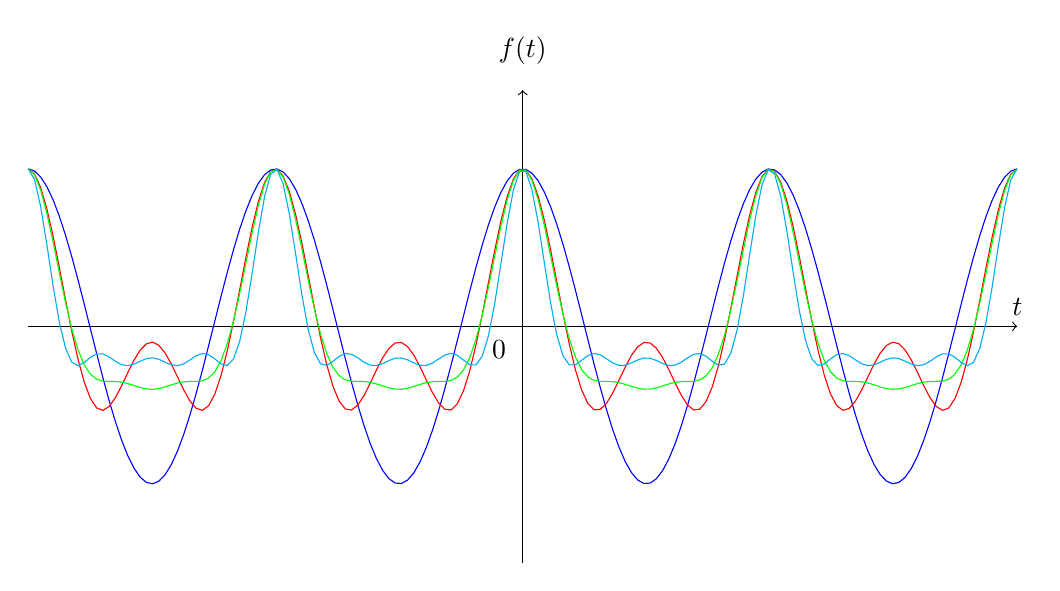
\begin{tikzpicture}

	\draw[->] (-6.28,0)-- (6.28,0);
\draw (-0.3,-0.3) node {0};
\draw[->] (0,-3)-- (0,3);
\draw (2*pi,0.25) node {$t$};
\draw (0,3.5) node {$f(t)$};
%\draw (4.5,-0.3) node {1};

%\draw[thick,blue] (0,0)-- (2.5,0);
%\draw[thick,blue] (2.5,0)-- (4.5,2);
%\draw[thick,blue] (2.5,2)-- (5,2);
\draw[domain=-6.28:6.28,color=blue,samples=160] plot (\x,{2*cos(2*\x r)});
	
	\draw[domain=-6.28:6.28,color=red,samples=160] plot (\x,{2*(0.55*cos(2*\x r)+ 0.45*cos(2*2*\x r))});
	
	\draw[domain=-6.28:6.28,color=green,samples=160] plot (\x,{2*(0.6*cos(2*\x r)+ 0.3*cos(2*2*\x r)+0.1*cos(2*3*\x r))});

		\draw[domain=-6.28:6.28,color=cyan,samples=160] plot (\x,{2*(0.4*cos(2*\x r)+ 0.3*cos(2*2*\x r)+0.2*cos(2*3*\x r) +0.1*cos(2*4*\x r) )});

	\end{tikzpicture}
\end{center}

On a représenté graphiquement les quatre fonctions précédentes dans la figure ci-dessus. On va maintenant représenter les coefficients de leur série de Fourier dans un graphique comprenant la fréquence de l'harmonique en abscisses et son amplitude en ordonnée.

\begin{center}
\begin{tikzpicture}

	\draw[->] (0,0)-- (5,0);
\draw (-0.3,-0.3) node {0};
\draw[->] (0,0)-- (0,3);
\draw (5.1,0.25) node {$f$};
\draw (0,3.5) node {$a_n(f)$};
%\draw (4.5,-0.3) node {1};

\draw[thick,blue] (1,0)-- (1,2);
\draw (1.1,-0.4) node {$\frac{1}{\pi}$};

\draw[thick,red] (1.05,0)-- (1.05,2.5*0.55);
\draw[thick,red] (2.05,0)-- (2.05,2.5*0.45);
\draw (2.1,-0.4) node {$\frac{2}{\pi}$};

\draw[thick,green] (1.1,0)-- (1.1,2.5*0.6);
\draw[thick,green] (2.1,0)-- (2.1,2.5*0.3);
\draw[thick,green] (3.1,0)-- (3.1,2.5*0.1);
\draw (3.1,-0.4) node {$\frac{3}{\pi}$};

\draw[thick,cyan] (1.15,0)-- (1.15,2.5*0.4);
\draw[thick,cyan] (2.15,0)-- (2.15,2.5*0.3);
\draw[thick,cyan] (3.15,0)-- (3.15,2.5*0.2);
\draw[thick,cyan] (4.15,0)-- (4.15,2.5*0.1);
\draw (4.1,-0.4) node {$\frac{4}{\pi}$};

	\end{tikzpicture}
\end{center}

Un premier point important est qu'on a construit des signaux uniquement autour de fonctions cosinus. On peut donc spécifier intégralement le signal en ne traçant que les coefficients $a_n(f)$, mais dans le cas général, il faudrait également tracer les coefficients $b_n(f)$, qui sont ici tous nuls.\\

On note que puisqu'on a utilisé uniquement des cosinus dans la construction du signal, tous les signaux sont "en phase" au sens où les maxima de chaque composantes vont se superposer, ce qui se voit notamment autour de zéro.\\

C'est ce principe de synthèse qui est parfois utilisé dans les générateurs de fonctions en électronique.\\

Une dernière chose importante: La représentation graphique ici ne sera pas qualifié de spectre. Ce terme renvoie à un objet mathématiques bien défini et bien que le lien conceptuel soit assez intuitif, on ne peut rigoureusement parler de spectre pour le graphique précédent.\\

\subsubsection{Transformée de Fourier}

\textbf{Question: Quelle est pour vous le lien entre transformée de Laplace et transformée de Fourier}

Puisqu'on a défini auparavant la transformée de Laplace on peut définir la transformée de Fourier en se basant sur cette dernière. On rappelle la définition de la transformée de Laplace :

\[L{g}(p) = \int^{\infty}_{-\infty} g(t) e^{-pt} \; dt\]\\ 

On peut alors définir la transformée de Fourier de la manière suivante:

\[TF{g}(\omega) = \int^{\infty}_{-\infty} g(t) e^{-j\omega t} \; dt\]\\

On remplace alors la variable de Laplace, $p$ par  $j \omega = 2 \pi j f$ où $f$  est la fréquence qui est homogène à l'inverse d'un temps.\\

La différence entre Fourier et Laplace se situe surtout au niveau du type  d'analyse effectuée. La méthode de Fourier est généralement plus restrictive du fait de sa forme mathématique. Celle-ci se prête notamment mieux aux analyses harmoniques.\\

On peut notamment en avoir l'intuition si on regarde la fonction qui sert à "projeter" le signal $g(t)$ dans l'espace dual. Dans le cas de Laplace, la fonction $e^{-pt}$ peut se décomposer comme $e^{-at}e^{-jbt}$. Le terme de droite est une fonction exponentielle décroissante de la variable temporelle et le membre de gauche est une exponentielle complexe qui peut se réécrire comme une fonction sinusoïdale. Ce qui veut dire que dans le cas de la transformée de Fourier (qui ne conserve que le terme de gauche) l'analyse sera "tournée vers" les fonctions de ce type, et c'est pour cette raison que la transformée de Fourier est un des outils de base de l'analyse harmonique. \\

\textbf{Question: Quelle est pour vous le lien entre les séries de Fourier et transformée de Fourier?} \\

Dans la partie précédente, on a introduit les séries de Fourier et on a construit un graphique où on reportait les coefficients de chaque harmonique. Cela dit, il a été très clairement spécifié que cet outil s'appliquait UNIQUEMENT aux fonctions périodiques. Cette restriction théorique complique l'application des séries de Fourier et l'analyse des harmoniques à beaucoup de signaux "physiques".\\

Sur un plan conceptuel, la transformée de Fourier est une généralisation aux fonctions non-périodiques du développement en série de Fourier. Pour mieux comprendre comment cette généralisation et ses implications on va reprendre l'exemple de nos quatre sommes de cosinus.\\

\textbf{Calculer la transformée de Fourier des quatre fonctions suivantes:}
\begin{enumerate}
\item $g_1(t) = \cos(2 t)$
\item $g_2(t) = 0.55 \cos(2 t) + 0.45 \cos(4 t)$
\item $g_3(t) = 0.6 \cos(2 t) + 0.3 \cos(4 t) + 0.1 \cos(6 t)$
\item $g_4(t) = 0.4 \cos(2 t) + 0.3 \cos(4 t) + 0.2 \cos(6 t) + 0.1 \cos(8 t) $
\end{enumerate} 
On rappelle que la période de toutes ces fonctions est $\pi$

\paragraph{1. $f_1(t) = \cos(2 t)$}
 \[TF{g_1}(f) = \int^{\infty}_{-\infty} g_1(t) e^{-2\pi j f t} \; dt\]
 \[TF{g_1}(f) = \int^{\infty}_{-\infty} \cos(2 t) e^{-2\pi j f t} \; dt\]
\[TF{g_1}(f) = \int^{\infty}_{-\infty} (\frac{e^{2jt} +  e^{-2jt}}{2}) e^{-2\pi j f t} \; dt\]
\[TF{g_1}(f) = \int^{\infty}_{-\infty} (\frac{e^{-j(2 \pi f -2)t}}{2}) \; dt + \int^{\infty}_{-\infty} (\frac{e^{-j(2 \pi f +2)t}}{2}) \; dt\]

pour aller plus loin il faut savoir que : 

 \[\int^{\infty}_{-\infty}  e^{-2\pi j f t} \; dt = \delta(f)\]
 
Ce qui mène à :

\[TF{g_1}(f) = \frac{1}{2}(\delta(f+2) + \delta(f-2))\]

\paragraph{2. $g_2(t) = 0.55 \cos(2 t) + 0.45 \cos(4 t)$}
En repartant du résultat précédent on en déduit le résultat suivant:

\[TF{g_2}(f) = \frac{0.55}{2}(\delta(f+2) + \delta(f-2)) + \frac{0.45}{2}(\delta(f+4) + \delta(f-4))\]

On a donc la somme de 4 diracs, 2 par composantes.

\paragraph{3. $g_3(t) = 0.6 \cos(2 t) + 0.3 \cos(4 t) + 0.1 \cos(6 t)$}
En repartant du résultat précédent on en déduit le résultat suivant:

\[TF{g_3}(f) = \frac{0.6}{2}(\delta(f+2) + \delta(f-2)) + \frac{0.3}{2}(\delta(f+4) + \delta(f-4)) + \frac{0.1}{2}(\delta(f+6) + \delta(f-6))\]

\paragraph{4. $g_4(t) = 0.4 \cos(2 t) + 0.3 \cos(4 t) + 0.2 \cos(6 t) + 0.1 \cos(8 t)$}
En repartant du résultat précédent on en déduit le résultat suivant:

\[TF{g_4}(f) = \frac{0.4}{2}(\delta(f+2) + \delta(f-2)) + \frac{0.3}{2}(\delta(f+4) + \delta(f-4)) + \frac{0.2}{2}(\delta(f+6) + \delta(f-6))\]
\[ + \frac{0.1}{2}(\delta(f+8) + \delta(f-8)) \]


On peut alors tracer le \textbf{spectre} de ces fonctions. Le spectre d'un signal est toujours représenté par deux graphes. Le premier, et celui qu'on se figure plus fréquemment quand on parle de spectre est le spectre en amplitude du signal, qui équivaut au module de la transformée de Fourier du signal.\\

\underline{\textbf{Rappel:}} Soit un complexe $z$ = $a + ib$, alors le module de $z$ est un réel $\rho$ défini comme :

\[ \rho = \sqrt{a^2 + b^2}  \]

On définit également l'argument de $z$ est un réel $\theta$ défini comme:

\[ \theta =  \arctan\frac{b}{a} = \arccos{\frac{a}{\rho}} = \arcsin{\frac{b}{\rho}} \] 

On peut alors écrire le complexe $z$ sous la forme $\rho e^{i \theta}$\\s

Donc si on trace le module du spectre de nos fonctions sinusoïdales précédentes, on obtient le spectre suivant. On note quand dans le cas de la  transformée de Fourier le spectre comporte des composantes positives ET négatives en fréquences ce qui n'était pas le cas dans le représentation en série de Fourier. 
\begin{center}
\begin{tikzpicture}

	\draw[->] (-5,0)-- (5,0);
\draw (-0,-0.3) node {0};
\draw[->] (0,0)-- (0,3);
\draw (5.1,0.25) node {$f$};
\draw (0,3.5) node {$|S(f)|$};
%\draw (4.5,-0.3) node {1};

\draw[thick,blue] (1,0)-- (1,2);
\draw (1.1,-0.4) node {$\frac{1}{\pi}$};

\draw[thick,red] (1.05,0)-- (1.05,2.5*0.55);
\draw[thick,red] (2.05,0)-- (2.05,2.5*0.45);
\draw (2.1,-0.4) node {$\frac{2}{\pi}$};

\draw[thick,green] (1.1,0)-- (1.1,2.5*0.6);
\draw[thick,green] (2.1,0)-- (2.1,2.5*0.3);
\draw[thick,green] (3.1,0)-- (3.1,2.5*0.1);
\draw (3.1,-0.4) node {$\frac{3}{\pi}$};

\draw[thick,cyan] (1.15,0)-- (1.15,2.5*0.4);
\draw[thick,cyan] (2.15,0)-- (2.15,2.5*0.3);
\draw[thick,cyan] (3.15,0)-- (3.15,2.5*0.2);
\draw[thick,cyan] (4.15,0)-- (4.15,2.5*0.1);
\draw (4.1,-0.4) node {$\frac{4}{\pi}$};

\draw[thick,blue] (-1,0)-- (-1,2);
\draw (-1.1,-0.4) node {$\frac{1}{\pi}$};

\draw[thick,red] (-1.05,0)-- (-1.05,2.5*0.55);
\draw[thick,red] (-2.05,0)-- (-2.05,2.5*0.45);
\draw (-2.1,-0.4) node {$\frac{2}{\pi}$};

\draw[thick,green] (-1.1,0)-- (-1.1,2.5*0.6);
\draw[thick,green] (-2.1,0)-- (-2.1,2.5*0.3);
\draw[thick,green] (-3.1,0)-- (-3.1,2.5*0.1);
\draw (-3.1,-0.4) node {$\frac{3}{\pi}$};

\draw[thick,cyan] (-1.15,0)-- (-1.15,2.5*0.4);
\draw[thick,cyan] (-2.15,0)-- (-2.15,2.5*0.3);
\draw[thick,cyan] (-3.15,0)-- (-3.15,2.5*0.2);
\draw[thick,cyan] (-4.15,0)-- (-4.15,2.5*0.1);
\draw (-4.1,-0.4) node {$\frac{4}{\pi}$};

	\end{tikzpicture}
\end{center}

Ici on a représenté le module du spectre mais pas son argument. On a donc un spectre d'amplitude mais pas un spectre de phase or ces deux aspects sont importants dans la représentation d'un signal c'est pourquoi on doit se pencher sur un second exemple pour pouvoir mettre en évidence cette notion de phase.\\

On va donc partir d'un second signal :

\[ g_5(t) = \cos(2 t) + 0.45 \cos(4 t + \frac{\pi}{3}) \] 

Il s'agit de la fonction $g_2(t)$ mais légèrement modifiée. On a introduit un déphasage de $\frac{\pi}{3}$. On peut visualiser ce déphasage dans la figure où on a représenté les fonctions $g_2(t)$ et $g_5(t)$.


\begin{center}
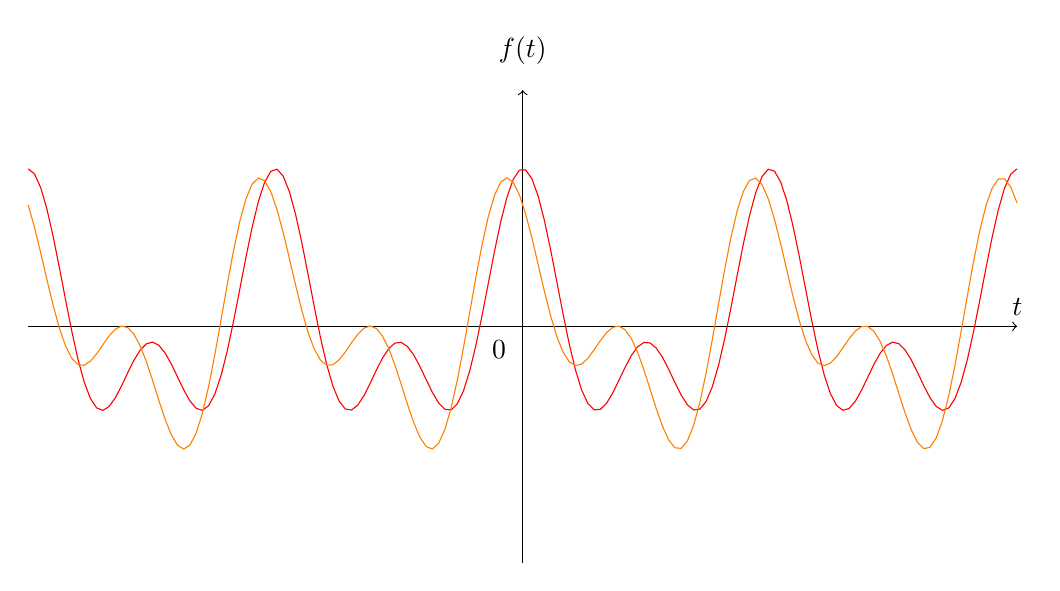
\begin{tikzpicture}

	\draw[->] (-6.28,0)-- (6.28,0);
\draw (-0.3,-0.3) node {0};
\draw[->] (0,-3)-- (0,3);
\draw (2*pi,0.25) node {$t$};
\draw (0,3.5) node {$f(t)$};
%\draw (4.5,-0.3) node {1};

%\draw[thick,blue] (0,0)-- (2.5,0);
%\draw[thick,blue] (2.5,0)-- (4.5,2);
%\draw[thick,blue] (2.5,2)-- (5,2);
	\draw[domain=-6.28:6.28,color=red,samples=160] plot (\x,{2*(0.55*cos(2*\x r)+ 0.45*cos(2*2*\x r))});
	
		\draw[domain=-6.28:6.28,color=orange,samples=160] plot (\x,{2*(0.55*cos(2*\x r)+ 0.45*cos(2*2*(\x+3.14/12) r))});
	
	\end{tikzpicture}
\end{center}
On voit que l'ajout du terme de déphasage a un impact visible sur la forme de la fonction et que le déphasage de la composante "haute fréquence" change la forme du signal.\\

On rappelle la transformée de Fourier du signal précédent :

\[ TF{g_2}(f) =   \frac{0.55}{2}(\delta(f+2) + \delta(f-2)) + \frac{0.45}{2}(\delta(f+4) + \delta(f-4))\]

On peut alors en déduire facilement la transformée de Fourier de $g_5(t)$

\[ TF{g_5}(f) =   \frac{0.55}{2}(\delta(f+2) + \delta(f-2)) + \frac{0.45}{2}(\delta(f+4) + \delta(f-4))e^{-2 j \pi \frac{pi}{3} f }\]

Si $TF{g_2}(f)$ était une fonction réelle (pas de partie complexe), $TF{g_5}(f)$ a clairement une partie imaginaire non nulle. On note également que dans ce cas le module et l'argument sont déjà présentées de façon évidente.\\

Le module des deux fonctions est identique. En effet, on sait que $|e^{-2 j \pi \frac{pi}{3} f }|=1$. Et donc, les modules des deux fonctions sont identiques. Ce qui distingue les deux fonctions dans ce cas est leur phase, soit l'argument de la transformée de Fourier.  Et effet, 

\[ arg(TF{g_2}(f)) =   0 \]

et

\[ arg(TF{g_5}(f)) =   -\frac{2}{3} f\]

On peut alors représenter graphiquement la phase des deux fonctions

\begin{center}
\begin{tikzpicture}

	\draw[->] (-5,0)-- (5,0);
\draw (-0.3,-0.3) node {0};
\draw[->] (0,-3)-- (0,3);
\draw (5.1,0.25) node {$f$};
\draw (0,3.5) node {$arg(S(f))$};
%\draw (4.5,-0.3) node {1};

\draw[thick,red] (-5,0)-- (5,0);

\draw[thick,orange] (-4.9,3.23)-- (4.9,-3.23);
	\end{tikzpicture}
\end{center}

Cette exemple démontre bien l'importance générale de la phase des signaux et pas seulement de leur spectre d'amplitude qui est souvent ce que les étudiants gardent à l'esprit lorsqu'on leur présente ces notions. Cette notion de phase reprendra de l'importance plus tard lorsqu'on présentera certains types de filtres.

\subsection{Signaux numériques}

\textbf{Question: En quoi consiste la numérisation d'un signal ?} \\

La numérisation d'un signal analogique initial est constitué de deux parties: L'échantillonnage et le codage. Les deux prochaines sous-parties traiteront de chacune de ces notions.

\subsubsection{Codage}

\textbf{Question: Que vous évoque la notion de codage ?} \\

Le codage consiste à \textbf{quantifier} le signal avec une \textbf{dynamique} donnée. Un exemple simple est celui d'une fonction rampe $r(t)$.\\

\begin{center}
\begin{tikzpicture}

	\draw[->] (-4,0)-- (4,0);
\draw (0.3,-0.3) node {0};
\draw[->] (0,-3.2)-- (0,3.2);
\draw (4.1,0.25) node {$t$};
\draw (0,3.5) node {$r(t)$};

\draw (1,-0.1)-- (1,0.1);
\draw (1.0,-0.3) node {1};
\draw (2,-0.1)-- (2,0.1);
\draw (2.0,-0.3) node {2};
\draw (3,-0.1)-- (3,0.1);
\draw (3.0,-0.3) node {3};

\draw (-1,-0.1)-- (-1,0.1);
\draw (-1.0,0.3) node {-1};
\draw (-2,-0.1)-- (-2,0.1);
\draw (-2.0,0.3) node {-2};
\draw (-3,-0.1)-- (-3,0.1);
\draw (-3.0,0.3) node {-3};

\draw (-0.1,1)-- (0.1,1);
\draw (-0.3,1) node {1};
\draw (-0.1,2)-- (0.1,2);
\draw (-0.3,2) node {2};
\draw (-0.1,3)-- (0.1,3);
\draw (-0.3,3) node {3};

\draw (-0.1,-1)-- (0.1,-1);
\draw (0.3,-1) node {-1};
\draw (-0.1,-2)-- (0.1,-2);
\draw (0.3,-2) node {-2};
\draw (-0.1,-3)-- (0.1,-3);
\draw (0.3,-3) node {-3};

%r(t)
\draw[thick,blue] (-3,-3)-- (3,3);

\draw[thick,dashed,red] (-3,-3)-- (-2,-3);
\draw[thick,dashed,red] (-2,-3)-- (-2,-2);
\draw[thick,dashed,red] (-2,-2)-- (-1,-2);
\draw[thick,dashed,red] (-1,-2)-- (-1,-1);
\draw[thick,dashed,red] (-1,-1)-- (-0,-1);
\draw[thick,dashed,red] (-0,-1)-- (-0,-0);
\draw[thick,dashed,red] (-0,-0)-- (1,-0);
\draw[thick,dashed,red] (1,0)-- (1,1);
\draw[thick,dashed,red] (1,1)-- (2,1);
\draw[thick,dashed,red] (2,1)-- (2,2);
\draw[thick,dashed,red] (2,2)-- (3,2);
\draw[thick,dashed,red] (3,2)-- (3,3);

\draw[thick,dashed,green] (-3,-2)-- (-2,-2);
\draw[thick,dashed,green] (-3,-3)-- (-3,-2);
\draw[thick,dashed,green] (-2,-1)-- (-1,-1);
\draw[thick,dashed,green] (-2,-2)-- (-2,-1);
\draw[thick,dashed,green] (-1,-0)-- (-0,-0);
\draw[thick,dashed,green] (-1,-1)-- (-1,0);
\draw[thick,dashed,green] (-0,1)-- (1,1);
\draw[thick,dashed,green] (0,0)-- (0,1);
\draw[thick,dashed,green] (1,2)-- (2,2);
\draw[thick,dashed,green] (1,1)-- (1,2);
\draw[thick,dashed,green] (2,3)-- (3,3);
\draw[thick,dashed,green] (2,2)-- (2,3);
	\end{tikzpicture}
\end{center}

On voit dans la figure précédente deux exemples de quantification de la fonction rampe avec une \textbf{amplitude de crête} de 3 unités et un \textbf{échelon de quantification} d'une unité Dans un cas, on échantillonne par arrondi (vert) et dans l'autre on arrondit par troncature (rouge). On peut aussi imaginer un cas intermédiaire où la valeur de quantification correspondrait au milieu de l'intervalle.\\

Généralement, le codage se fait sur des nombres binaires. le nombre de valeurs disponibles est alors généralement donné par le nombre de bit utilisé pour le codage.\\

\textbf{Exercice: Si on code un signal d'une amplitude de crête de 5 volts sur 4 bits, quelle est la valeur de l'échelon de quantification ?}

4 bits binaires permettent de représenter 16 valeurs. L'intervalle [-5; 5] couvre 10 V au total. La solution la plus directe est de diviser la gamme en 10 secteurs égaux et de faire correspondre une des 16 valeurs binaires à chacun. Les secteurs ont une étendue de 0.625 V chacun et on peut diviser la gamme en 2N secteurs.

\begin{table}[h!]
\begin{center}
\begin{tabular}{|p{20mm}|p{10mm}|p{25mm}|}
 \hline
 code binaire &  valeur & amplitude \\
 \hline
 0000 & 0 &  [-5.000;-4.375] \\
 \hline
 0001 & 1 & [-4.375; -3.750]\\
 \hline
 0010 & 2 & [-3.750;-3.125]\\
 \hline
 0011 & 3 & [-3.125;-2.500]\\
 \hline
 0100 & 4 & [-2.500;-1.875]\\
 \hline
 0101 & 5 & [-1.875;-1.250]\\
 \hline
 0110 & 6 & [-1.250;-0.625]\\
 \hline
 0111 & 7 & [-0.625;0.000]\\
 \hline
 1000 & 8 &  [0.000;0.625]\\
 \hline
 1001 & 9 &  [0.625;1.250]\\
 \hline
 1010 & 10 & [1.250;1.875]\\
 \hline
 1011 & 11 & [1.875;2.500]\\
 \hline
 1100 & 12 & [2.500;3.125]\\
 \hline
 1101 & 13 & [3.125;3.750]\\
 \hline
 1110 & 14 & [3.750;4.375]\\
 \hline
 1111 & 15 & [4.375;5.000]\\
 \hline 
\end{tabular}
\end{center}
\end{table}

Le principe présenté dans la figure précédente s'applique de nouveau ici puisque chaque intervalle ne correspondra qu'à une valeur finale qui peut être sa borne inférieure, sa borne supérieure, ou une valeur intermédiaire. Mais il est important de comprendre qu'à ce stade on a aucun moyen de connaître la valeur plus précisément que ce que permet l'échelon de quantification.\\


L'approximation systématique du au codage induit une erreur et donc un bruit de quantification. Ce bruit de quantification dépend donc de paramètres très important du processus de codage. L'amplitude de codage, et l'échelon de quantification.\\

\subsubsection{L'échantillonnage}

\textbf{Question : En quoi consiste pour vous l'opération d'échantillonnage ?}

D'après le livre de Maurice Bellanger : "L’échantillonnage consiste à représenter un signal fonction du temps $s(t)$ par ses
valeurs $s(nT_e)$ à des instants multiples entiers d’une durée $T_e$, appelée période d’échantillonnage."\\

Mathématiquement, l'opération d'échantillonnage s'appuie sur la distribution appelée "peigne de Dirac" et qui est définie comme suit: 

\[ u_{T_e}(t) = \sum_{n = -\infty}^{\infty} \delta(t-nT_e) \]\\

Le signal échantillonné avec une période $T_e$ peut alors s'exprimer comme le produit $u_{T_e}(t) s(t)$.\\

\begin{center}
\begin{tikzpicture}

	\draw[->] (-5,0)-- (5,0);
\draw (-0.3,-0.3) node {0};
\draw[->] (0,-3)-- (0,3);
\draw (5.1,0.25) node {$f$};
\draw (0,3.5) node {$s(t)$};
%\draw (4.5,-0.3) node {1};

\draw[domain=-4.9:4.9,color=blue,samples=160] plot (\x,{2*(0.55*cos(2*\x r)+ 0.45*cos(2*2*(\x+3.14/12) r))});
	\end{tikzpicture}
\end{center}

\begin{center}
\begin{tikzpicture}

	\draw[->] (-5,0)-- (5,0);
\draw (-0.3,-0.3) node {0};
\draw[->] (0,-3)-- (0,3);
\draw (5.1,0.25) node {$f$};
\draw (0,3.5) node {$u_{T_e}(t)$};
%\draw (4.5,-0.3) node {1};

\draw[thick,blue] (-4,-0)-- (-4,1);
\draw[thick,blue] (-3,-0)-- (-3,1);
\draw[thick,blue] (-2,-0)-- (-2,1);
\draw[thick,blue] (-1,-0)-- (-1,1);
\draw[thick,blue] (0,-0)-- (0,1);
\draw[thick,blue] (1,-0)-- (1,1);
\draw[thick,blue] (2,-0)-- (2,1);
\draw[thick,blue] (3,-0)-- (3,1);
\draw[thick,blue] (4,-0)-- (4,1);
	\end{tikzpicture}
\end{center}

\begin{center}
\begin{tikzpicture}

	\draw[->] (-5,0)-- (5,0);
\draw (-0.3,-0.3) node {0};
\draw[->] (0,-3)-- (0,3);
\draw (5.1,0.25) node {$f$};
\draw (0,3.5) node {$u_{T_{e}}(t)s(t)$};
%\draw (4.5,-0.3) node {1};

\draw[dashed,domain=-4.9:4.9,color=blue,samples=160] plot (\x,{2*(0.55*cos(2*\x r)+ 0.45*cos(2*2*(\x+3.14/12) r))});

\draw[thick,blue] (-4,-0)-- (-4,-0.9);
\draw[thick,blue] (-3,-0)-- (-3,1);
\draw[thick,blue] (-2,-0)-- (-2,0);
\draw[thick,blue] (-1,-0)-- (-1,-1.25);
\draw[thick,blue] (0,-0)-- (0,1.3);
\draw[thick,blue] (1,-0)-- (1,-0.15);
\draw[thick,blue] (2,-0)-- (2,-1.5);
\draw[thick,blue] (3,-0)-- (3,1.8);
\draw[thick,blue] (4,-0)-- (4,-0.35);
	\end{tikzpicture}
\end{center}

Une des premières choses à aborder dans ce cas est l'impact de l'opération d'échantillonnage sur le spectre du signal:\\

\[ TF (\sum_{n = -\infty}^{\infty} s(t)\delta(t-nT_e)) = \sum_{n = -\infty}^{\infty} TF(s(t)\delta(t-nT_e) ) \]

\[ \sum_{n = -\infty}^{\infty} TF(s(t)\delta(t-nT_e) ) = \sum_{n = -\infty}^{\infty} S(f) \star e^{- 2j\pi n T_e f} \]\\

Pour aller plus loin il faut savoir que : 

\[ \sum_{n = -\infty}^{\infty} e^{- 2j\pi n T_e f} = \frac{1}{T_e} \sum_{n = -\infty}^{\infty} \delta(f - \frac{n}{T}) \]\\

Et que 

\[\delta \star \phi = \phi \]

Ce qui mène à 

\[ TF (\sum_{n = -\infty}^{\infty} s(t)\delta(t-nT_e)) = \frac{1}{T}\sum_{n = -\infty}^{\infty} S(f) \star \delta(f - \frac{n}{T_e})\]

La dernière expression traduit le fait que le spectre se répète dans l'espace des fréquences avec une période de $\frac{1}{T_e}$.\\

On va continuer avec l'exemple de la fonction $ g_5(t) = \cos(2 t) + 0.45 \cos(4 t + \frac{\pi}{3})$ dont on retrace le module du spectre dans  la figure suivante.

\begin{center}
\begin{tikzpicture}

	\draw[->] (-5,0)-- (5,0);
\draw (-0,-0.3) node {0};
\draw[->] (0,0)-- (0,3);
\draw (5.1,0.25) node {$f$};
\draw (0,3.5) node {$|S(f)|$};
%\draw (4.5,-0.3) node {1};


\draw[thick,blue] (1.05,0)-- (1.05,2.5*0.55);
\draw[thick,blue] (2.05,0)-- (2.05,2.5*0.45);
\draw (2.1,-0.4) node {$\frac{2}{\pi}$};
\draw (1.1,-0.4) node {$\frac{1}{\pi}$};

\draw[thick,blue] (-1.05,0)-- (-1.05,2.5*0.55);
\draw[thick,blue] (-2.05,0)-- (-2.05,2.5*0.45);
\draw (-2.1,-0.4) node {$\frac{2}{\pi}$};
\draw (-1.1,-0.4) node {$\frac{1}{\pi}$};


	\end{tikzpicture}
\end{center}

\textbf{Question: Que doit-on avoir à l'esprit  lors du choix de la période d’échantillonnage ?}\\

Lors de l'échantillonnage, on doit conserver l'information, mais aussi optimiser la quantité de données à gérer dans la plupart des cas.\\

Le théorème de Nyquist-Shannon dit : \textbf{"La représentation discrète d'un signal exige des échantillons régulièrement espacés à une fréquence d'échantillonnage supérieure au double de la fréquence maximale présente dans ce signal."}\\

Visuellement, il faut se figurer que la fréquence la plus élevée dans la norme du spectre donne la largeur du spectre. Dans le domaine temporel, cela se comprend de la façon suivante la variation avec la plus petite échelle temporelle n'est conservée que si la période d'échantillonnage permet d'en isoler au moins 2 points.\\

Lors de l'échantillonnage, le spectre est répliqué avec sa largeur complète à TOUS les multiples de la fréquence d'échantillonnage.\\

\textbf{Question: Quelle est la gamme de fréquences d'échantillonnage garantissant le respect de Nyquist-Shannon pour le signal $g5(t)$?}\\

Dans le cas de la fonction $g_5(t) = \cos(2 t) + 0.45 \cos(4 t + \frac{\pi}{3})$, on a vu dans la figure précédente que le spectre en amplitude présente deux raies. la fréquence maximale correspond donc à celle de la 2e raie : $\frac{2}{\pi}$. Le double de cette fréquence maximale donne donc $f_e = \frac{4}{\pi}$, et donc une période de $\frac{\pi}{4}$\\

\begin{center}
\begin{tikzpicture}

	\draw[->] (-5,0)-- (5,0);
\draw (-0.3,-0.3) node {0};
\draw[->] (0,-3)-- (0,3);
\draw (5.1,0.25) node {$f$};
\draw (0,3.5) node {$u_{T_{e}}(t)s(t)$};
%\draw (4.5,-0.3) node {1};

\draw[dotted,domain=-4.9:4.9,color=blue,samples=160] plot (\x,{2*(0.55*cos(2*\x r)+ 0.45*cos(2*2*(\x+3.14/12) r))});

\draw[thick,blue] (-4.74,-0)-- (-4.74,-0.55);
\draw[thick,blue] (-3.95,-0)-- (-3.95,-0.60);
\draw[thick,blue] (-3.16,-0)-- (-3.16,1.6);
\draw[thick,blue] (-2.37,-0)-- (-2.37,-0.45);
\draw[thick,blue] (-1.58,-0)-- (-1.58,-0.65);
\draw[thick,blue] (-0.79,-0)-- (-0.79,-0.65);
\draw[thick,blue] (0,-0)-- (0,1.5);
\draw[thick,blue] (0.79,-0)-- (0.79,-0.45);
\draw[thick,blue] (1.58,-0)-- (1.58,-0.6);
\draw[thick,blue] (2.37,-0)-- (2.37,-0.25);
\draw[thick,blue] (3.16,-0)-- (3.16,1.55);
\draw[thick,blue] (3.95,-0)-- (3.95,-0.45);
\draw[thick,blue] (4.74,-0)-- (4.74,-0.7);

\draw[dashed,cyan] (-4.74,-0.55)-- (-3.95,-0.6)--(-3.95,-0.6)--(-3.16,1.6)--(-2.37,-0.45)--(-1.58,-0.65)--(-0.79,-0.65)--(0,1.5)--(0.79,-0.45)--(1.58,-0.6)--(2.37,-0.25)--(3.16,1.55)--(3.95,-0.45)--(4.74,-0.7);

	\end{tikzpicture}
\end{center}

On voit bien si on représente la fonction échantillonnée que le respect strict ou minimal de la condition de Nyquist-Shannon donne lieu à une reconstruction qui peut paraître assez éloignée de la fonction initiale.  
\\

On peut également représenter le spectre en amplitude du signal échantillonnée. On rappelle que l'échantillonnage à une fréquence consiste à périodiser le spectre en fréquence avec une période de $f_e$. On va donc représenter ce spectre en amplitude dans la figure suivante.\\

\begin{center}
\begin{tikzpicture}

	\draw[->] (-7,0)-- (7,0);
\draw (-0,-0.3) node {0};
\draw[->] (0,0)-- (0,3);
\draw (7.1,0.25) node {$f$};
\draw (0,3.5) node {$|S(f)|$};
%\draw (4.5,-0.3) node {1};


\draw[thick,blue] (1.05,0)-- (1.05,2.5*0.55);
\draw[thick,blue] (2.05,0)-- (2.05,2.5*0.45);
\draw (2.1,-0.4) node {$\frac{2}{\pi}$};
\draw (1.1,-0.4) node {$\frac{1}{\pi}$};

\draw[thick,blue] (-1.05,0)-- (-1.05,2.5*0.55);
\draw[thick,blue] (-2.05,0)-- (-2.05,2.5*0.45);
\draw (-2.1,-0.4) node {$-\frac{2}{\pi}$};
\draw (-1.1,-0.4) node {$-\frac{1}{\pi}$};


%replica 1
\draw[thick,cyan] (5.05,0)-- (5.05,2.5*0.55);
\draw[thick,cyan] (6.05,0)-- (6.05,2.5*0.45);
\draw (5.1,-0.4) node {$\frac{5}{\pi}$};
\draw (6.1,-0.4) node {$\frac{6}{\pi}$};

\draw[thick,cyan] (3.05,0)-- (3.05,2.5*0.55);
\draw[thick,cyan] (2.08,0)-- (2.08,2.5*0.45);
\draw (3.1,-0.4) node {$\frac{3}{\pi}$};
%\draw (2.1,-0.4) node {$\frac{1}{\pi}$};
\draw (4.1,-0.4) node {$\frac{4}{\pi}$};


%replica 2
\draw[thick,cyan] (-5.05,0)-- (-5.05,2.5*0.55);
\draw[thick,cyan] (-6.05,0)-- (-6.05,2.5*0.45);
\draw (-5.1,-0.4) node {$-\frac{5}{\pi}$};
\draw (-6.1,-0.4) node {$-\frac{6}{\pi}$};

\draw[thick,cyan] (-3.05,0)-- (-3.05,2.5*0.55);
\draw[thick,cyan] (-2.08,0)-- (-2.08,2.5*0.45);
\draw (-3.1,-0.4) node {$-\frac{3}{\pi}$};
%\draw (2.1,-0.4) node {$\frac{1}{\pi}$};
\draw (-4.1,-0.4) node {$-\frac{4}{\pi}$};


	\end{tikzpicture}
\end{center}

Le spectre en amplitude permet de comprendre la notion de \textbf{repliement spectral}. Si on respecte le théorème de Nyquist-Shannon strictement on voit que les extrémités des répliques dues à l'échantillonnage sont quasiment confondues. Et donc si on choisit une fréquence d'échantillonnage inférieure, on va se retrouver avec des spectres qui se mélangent. Dans le domaine temporel cela va évidemment correspondre à des échantillons ne permettant pas de capturer toutes les caractéristiques du signal.\\

\subsubsection{Propriétés des signaux échantillonnés: Cas usuels}
% Kronecker
% signal échelon 
% etc...

\subsection{La transformée en Z}
Une outil mathématique particulièrement important en traitement du signal/filtrage numérique est la transformée en Z .\\

\textbf{Question: Que vous évoque la notion de transformée en Z ?}\\

La transformée en Z est définie de la façon suivante :

\[\sum_{n = 0}^{\infty} s_{T_e}(n) z^{-n}\] 

On la compare généralement à la transformée de Laplace. L'intégrale (somme continue) est remplacée par une somme discrète, et le terme exponentiel est remplacé par $z^{-n}$ C'est ce terme qui donne son à la transformée en Z. Tout comme $p$ dans la transformée de Laplace, $z$  est une variable \textbf{complexe}. Il est important de noter que le fait que la somme soit infinie oblige la variable $z$ à avoir un module inférieur à 1 pour converger.\\

La comparaison avec la transformée de Laplace vient surtout du fait que la transformée en Z a des propriétés sur des signaux discrets très similaires à celle de la transformée de Laplace pour les signaux continus. C'est ce qu'on va illustrer dans les sous-parties suivantes.\\

\subsubsection{Transformée en Z des fonctions usuelles}

\textbf{Exercice: Calculez les transformées en Z des quatre suites suivantes}
\begin{enumerate}
\item $\delta[n]$
\item $u[n]$
\item $nu[n]$
\item $sin(\omega_0 n)u(n)$
\end{enumerate} 

\textbf{1. $\delta[n]$}
\[\sum_{n = 0}^{\infty} \delta[n] z^{-n}\] \\

$\delta[n]$ est la suite définie comme prenant la valeur 1 pour l'échantillon d'index 0 et 0 sur tous les autres points. Donc,\\

\[\sum_{n = 0}^{\infty} \delta[n] z^{-n} = z^0 = 1 \]\\

\textbf{2. $u[n]$}

$u[n]$ est la suite définie comme prenant la valeur 1 pour l'échantillon d'index 0 et tous les suivants. Donc,\\

\[\sum_{n = 0}^{\infty} u[n] z^{-n} = \sum_{n = 0}^{\infty} z^{-n}  = \frac{1}{1-z^{-1}} \]\\

La dernière étape est un résultat connu sur la série géométrique convergente. Ce résultat n'est d'ailleurs vraie que si la valeur absolue ou le module de la raison de la suite (ici, $z$) est strictement inférieur à 1. 

\textbf{3. $nu[n]$}

 $nu[n]$ est l'équivalent discret de la fonction rampe.\\
 

\[\sum_{n = 0}^{\infty} n u[n] z^{-n} = \sum_{n = 0}^{\infty} n z^{-n}  = \frac{z^{-1}}{(1-z^{-1})^2} \]\\ 

Dans ce cas, la valeur de la somme peut se démontrer en utilisant une méthode analogue au cas précédent mais cette fois dans le cas d'une suite arithmético-géométrique.

%proof : https://en.wikipedia.org/wiki/Arithmetico-geometric_sequence#Sum_of_the_terms


\subsubsection{Propriétés de la transformée en Z}

\textbf{Exercice : démontrer la linéarité de la transformée en Z}\\

soit $x(n) = a x_1(n) + b x_2(n)$, alors,

\[X(z) = \sum_{n = 0}^{\infty} x(n) z^{-n}\] 

\[X(z) = \sum_{n = 0}^{\infty} (a x_1(n) + b x_2(n)) z^{-n}\] 

\[X(z) = a \sum_{n = 0}^{\infty} x_1(n)  z^{-n} + b \sum_{n = 0}^{\infty} x_2(n) \] 

\[X(z) = a X_1(z)+ b X_2(z) \] 

\textbf{Exercice : Calcular la trasnformée en Z de $x_1(t) \star x_2(t)$}\\


\subsection{La transformée de Fourier discrète (TFD)}

\textbf{Question: Que vous évoque la notion de transformée de Fourier Discrète ?}

Dans la sous-partie précédente on a présenté la transformée en Z. La transformée de Fourier discrète est une notion un peu différente.



\subsubsection{Les convertisseurs}

\subsection{Conclusion Rappels}
Dans cette section sur les fondamentaux, on a rappelé des définitions importantes en traitement du signal et on les replacés dans le contexte du traitement du signal numérique et des chaînes d'instrumentation.\\

On a rappelé les notions d'invariance dans le temps et de linéarité des filtres et leur importance dans l'établissement de la relation de convolution.\\

On a rappelé les définitions des transformées de Fourier et de Laplace, leur propriétés ainsi que quelques transformées usuelles par le biais d'exemple.\\

On a ensuite abordé les notions importantes de codage et d'échantillonnage pour passer un signal du domaine temporel continu au domaine temporel discret. On a pu voir l'impact de l'échantillonnage sur le spectre en amplitude et on a rappelé l'importance du théorème de Nyquist-Shannon. \\
pur finir on a discuté des propriétés particulières des signaux échantillonnés et on a les comparés à celles de signaux continus équivalents.\\




\end{document}